\documentclass[10pt,twocolumn]{article}

% ─── Packages ───────────────────────────────────────────────────────────────
\usepackage[margin=1in]{geometry}
\usepackage{amsmath,amssymb,amsthm}
\usepackage{graphicx}
\usepackage{booktabs}
%\usepackage{multirow}
\usepackage{xcolor}
\usepackage{hyperref}
\usepackage{algorithm}
\usepackage{algorithmic}
\usepackage{natbib}
\usepackage{subcaption}
\usepackage{float}
\usepackage[T1]{fontenc}

% ─── Macros ──────────────────────────────────────────────────────────────────
\newcommand{\todo}[1]{\textcolor{red}{\textbf{[TODO: #1]}}}
\newcommand{\wip}[1]{\textcolor{orange}{\textbf{[WIP: #1]}}}
\newcommand{\needdata}[1]{\textcolor{blue}{\textbf{[DATA NEEDED: #1]}}}
\newcommand{\mcpilot}{MC-PILOT}
\newcommand{\mcpilco}{MC-PILCO}
\newcommand{\ie}{\textit{i.e.}}
\newcommand{\eg}{\textit{e.g.}}

% ─── Theorem-like environments ───────────────────────────────────────────────
\newtheorem{proposition}{Proposition}
\newtheorem{remark}{Remark}

% ─── Title block ─────────────────────────────────────────────────────────────
\title{\textbf{Geometry, Exploration, and Noise:\\
A Diagnostic Study of Model-Based Reinforcement Learning\\
for Data-Efficient Robotic Throwing}}

\author{
  AR525 Group-3 \\
  Indian Institute of Technology Mandi \\
  \texttt{[author emails]}
}

\date{}

% ─────────────────────────────────────────────────────────────────────────────
\begin{document}
\maketitle

% ─── Abstract ────────────────────────────────────────────────────────────────
\begin{abstract}
Robotic throwing offers a path to fast, long-range manipulation in industrial settings,
but learning reliable release policies demands data efficiency: physical robots tolerate
only tens of trials before wear or safety constraints intervene.
\mcpilot{}~\cite{turcato2025mcpilot} addresses this via a Gaussian-process (GP) dynamics
model and a single-shot radial-basis-function (RBF) speed policy optimised with
Monte Carlo policy gradients,
achieving near-perfect target coverage in roughly ten throws on a Franka Panda arm.

We reproduce \mcpilot{} in an independent ballistic simulator, diagnose four non-obvious
silent failure modes in the original codebase, and conduct five experimental studies to
characterise the algorithm's robustness and portability.
From this diagnostic process we derive two portable design rules: a
\emph{lengthscale-to-range scaling rule} ($\ell_s \approx 0.15 \times
\text{target\_range}$) that prevents RBF blindness in narrow target domains, and a
\emph{stratified exploration policy} that provides seed-robust GP initialisation without
additional hardware trials.
We achieve 100\% hit rates across five release heights ($z \in \{0.0, 0.5, 1.0, 1.5,
2.0\}$\,m) and demonstrate arm-agnostic portability across three robot platforms (Franka
Panda, KUKA iiwa7, xArm6) through a decoupled architecture that separates RL from arm
kinematics.
We prove a \emph{zero-mean noise invariance theorem}---symmetric additive noise does not
shift the optimal policy mean, only biased noise is learnable---and validate it
empirically: a noise-aware policy achieves 100\% hit rate versus 0\% for a naive
baseline under 20\% velocity slip.
Finally, we present a wind robustness study revealing a counterintuitive
curse-of-dimensionality effect: blind GP policies outperform explicit wind-conditioned
policies across all three wind regimes in the low-data budget, and a closed-loop vision
pipeline (OpenCV HSV segmentation and YOLOv8n detection) that enables autonomous bin
targeting without pre-specified target coordinates.
\end{abstract}


% ─── Body sections ───────────────────────────────────────────────────────────
\section{Introduction}
\label{sec:introduction}

Robotic throwing extends the effective reach of a manipulator far beyond its kinematic
workspace, enabling rapid sorting, bin-to-bin transfer, and long-range placement without
additional actuators.
Industrial pick-and-throw cells can double throughput compared with pick-and-place
because the robot releases the object at high speed and immediately returns for the next
grasp while the projectile is still in flight~\cite{turcato2025mcpilot}.
Despite this appeal, practical deployment is bottlenecked by \emph{data efficiency}:
learning a reliable release policy on physical hardware must converge in tens of trials
rather than thousands, because each trial incurs wear, reconfiguration overhead, and
safety risk.
Standard model-free RL methods (\eg TossingBot~\cite{tossbot}) require orders of
magnitude more samples than this budget permits, motivating model-based approaches that
explicitly represent uncertainty and plan through it.

\mcpilot{}~\cite{turcato2025mcpilot} addresses this challenge by combining
\mcpilco{}~\cite{mcpilco}---a Gaussian-process (GP) dynamics model with Monte Carlo
policy gradients---with two throwing-specific modifications.
First, the policy is reduced to a single-shot speed map $\pi_\theta(\mathbf{P})$
that fires exactly once at $t{=}0$ given the target position $\mathbf{P}$, eliminating
the need for closed-loop feedback during flight.
Second, gripper release delay is estimated by Bayesian Optimisation, compensating for
systematic timing errors that would otherwise corrupt every trajectory.
The augmented state $\tilde{\mathbf{x}} = [\mathbf{x},\, \mathbf{P}]$ lets the GP learn
geometry-conditioned corrections, and the RBF policy network enables smooth interpolation
across the target workspace.
On a Franka Panda arm with a Gazebo/ROS simulator, \mcpilot{} reaches near-100\% target
coverage in approximately ten physical throws.

Despite these results, several practical gaps remain unexplored.
\textbf{(1) Geometry sensitivity.}
The published hyperparameters are calibrated to a single release height and target range;
na\"ive transfer to different heights silently degrades performance.
\textbf{(2) Arm portability.}
The paper is locked to a single robot platform; it is unknown whether the algorithm's
data-efficiency transfers to other manipulators.
\textbf{(3) Noise structure.}
Physical robots exhibit velocity slip, timing jitter, and gripper compliance whose
statistical structure differs from zero-mean additive noise; the learnability of each
noise type is not characterised.
\textbf{(4) Environmental disturbances.}
Outdoor or warehouse environments introduce wind, yet the algorithm has not been tested
under ambient airflow.
\textbf{(5) Perception.}
Deployment requires autonomous bin detection; the original work pre-specifies target
coordinates rather than detecting them visually.
\textbf{(6) Reproducibility.}
The original implementation requires Gazebo and ROS, limiting accessibility; the
algorithm's core physics is ballistic and admits a lightweight numpy simulation.

\paragraph{Contributions.}
\begin{enumerate}
  \item \textbf{Independent simulation reproduction.}
        A self-contained ballistic simulator and PyBullet visualiser that replicate
        \mcpilot{} without Gazebo or ROS, with all adaptation decisions documented.

  \item \textbf{Four diagnosed failure modes.}
        Systematic identification and correction of four non-obvious silent failure modes:
        broken gradient path, post-landing GP hallucination, cost-lengthscale saturation,
        and simulation-horizon unit mismatch.

  \item \textbf{Two convergence rules.}
        (a) The \emph{lengthscale-to-range scaling rule} $\ell_s \approx 0.15 \times
        \text{target\_range}$ prevents RBF blindness across all tested geometries.
        (b) The \emph{stratified exploration rule} guarantees seed-robust GP coverage
        with no additional hardware throws.

  \item \textbf{Release-height generalisation.}
        100\% hit rates across all five tested heights ($z \in \{0.0, 0.5, 1.0, 1.5,
        2.0\}$\,m) with mean landing errors below 35\,mm.

  \item \textbf{Multi-arm portability.}
        100\% commanded-velocity hit rates on Franka Panda, KUKA iiwa7, and xArm6
        without any retraining, demonstrating arm-agnostic RL through a decoupled
        architecture.

  \item \textbf{Zero-mean noise invariance theorem.}
        Theorem~\ref{thm:zeromean} proves that symmetric zero-mean noise does not shift
        the optimal policy, with an experimental demonstration of 100\% vs.\ 0\%
        hit rate for noise-aware vs.\ naive policies under 20\% velocity slip.

  \item \textbf{Wind robustness study.}
        A full pipeline extension (air-relative drag, 8-D$\to$11-D state augmentation,
        policy and GP updates) and the counterintuitive finding that blind GP policies
        outperform wind-aware policies in all three wind regimes within the 15-trial budget.

  \item \textbf{Closed-loop vision result.}
        We show that colour-based (OpenCV HSV) and learning-based (YOLOv8n on 800
        synthetic PyBullet images) detection pipelines both produce target estimates
        accurate enough to drive the trained policy to successful throws, with the
        near-face depth bias correctable by a geometric $2R/\pi$ shift.
        This establishes that the trained policy is robust to centimetre-level
        target-position estimation error.
\end{enumerate}

\paragraph{Paper structure.}
Section~\ref{sec:background} provides an expanded treatment of MC-PILCO and the
\mcpilot{} formulation.
Section~\ref{sec:system} describes the system architecture.
Section~\ref{sec:implementation} details the four diagnosed failure modes.
Section~\ref{sec:convergence} presents the two convergence rules.
Sections~\ref{sec:study1}--\ref{sec:study5} present the five experimental studies.
Section~\ref{sec:discussion} synthesises findings.
Section~\ref{sec:conclusion} concludes.

\section{Background}
\label{sec:background}

\subsection{MC-PILCO}
\label{sec:background:mcpilco}

\mcpilco{}~\cite{mcpilco} is a model-based RL framework for continuous control that
couples a GP dynamics model with a Monte Carlo (MC) policy-gradient optimiser.
The GP is fit to observed transitions $(\mathbf{x}_t, \mathbf{u}_t) \to \mathbf{x}_{t+1}$
and maintains a posterior over residual corrections to a known nominal model.
At each policy update step, $M$ particles are propagated forward through the GP posterior
via the reparameterisation trick: each particle draws a function sample from the GP and
integrates the resulting ODE, yielding a set of stochastic rollouts that can be
differentiated with respect to policy parameters $\theta$.
The policy gradient is then

\begin{equation}
  \nabla_\theta J(\theta) = \nabla_\theta \mathbb{E}\!\left[
    \sum_{t=0}^{T} c(\tilde{\mathbf{x}}_t)
  \right] \approx \frac{1}{M}\sum_{m=1}^{M} \nabla_\theta \sum_{t=0}^{T}
  c(\tilde{\mathbf{x}}_t^{(m)}),
  \label{eq:mcpilco_gradient}
\end{equation}

where the reparameterisation ensures that the Monte Carlo samples are differentiable
through the GP posterior.
Sparse approximation via Subset of Data (SOD) keeps inference tractable as the dataset
grows across trials.

\subsection{MC-PILOT Modifications}
\label{sec:background:mcpilot}

\mcpilot{}~\cite{turcato2025mcpilot} adapts \mcpilco{} for the single-shot throwing
problem with two targeted modifications.

\paragraph{Augmented state.}
The robot state $\mathbf{x} = [\mathbf{p},\, \dot{\mathbf{p}}] \in \mathbb{R}^6$
(position and velocity) is augmented with the target location
$\mathbf{P} = (P_x, P_y) \in \mathbb{R}^2$ to form
$\tilde{\mathbf{x}} = [\mathbf{x},\, \mathbf{P}] \in \mathbb{R}^8$.
The GP learns per-timestep velocity corrections
$[\Delta v_x, \Delta v_y, \Delta v_z]$ conditioned on $\tilde{\mathbf{x}}$, enabling
geometry-conditioned residual compensation across the target workspace.

\paragraph{Single-shot policy.}
Because the projectile is in free flight after release, feedback control is neither
possible nor necessary.
The policy collapses to a single map from target position to release speed:

\begin{equation}
  \pi_\theta(\mathbf{P}) = \frac{u_M}{2}\!\left(
    \tanh\!\left(
      \sum_{i=1}^{N_b} w_i \exp\!\left(
        -\frac{\|\mathbf{a}_i - \mathbf{P}\|^2}{\ell_s^2}
      \right)
    \right) + 1
  \right),
  \label{eq:policy}
\end{equation}

where $u_M$ is the maximum allowable speed, $\{(\mathbf{a}_i, w_i)\}_{i=1}^{N_b}$ are
the $N_b$ RBF centres and weights (the trainable parameters $\theta$), and $\ell_s$ is
the lengthscale that controls the spatial extent of each basis function.
The $\tanh(\cdot) + 1$ construction squashes the output to $(0,\, u_M)$, enforcing
physical speed limits.

\paragraph{Landing cost.}
Performance is measured at the final timestep $T$ (the moment of landing) by a
Gaussian-shaped cost centred on the target:

\begin{equation}
  c(\tilde{\mathbf{x}}_T) = 1 - \exp\!\left(
    -\|\mathbf{p}_T - \mathbf{P}\|^2 \cdot \Sigma_c^{-1}
  \right),
  \label{eq:cost}
\end{equation}

where $\mathbf{p}_T \in \mathbb{R}^2$ is the ball landing position and $\Sigma_c$
controls the width of the acceptance region.
The policy objective is $J(\theta) = \mathbb{E}[c(\tilde{\mathbf{x}}_T)]$, minimised
by gradient descent through the MC rollouts.

\subsection{Aerodynamic Drag Model}
\label{sec:background:drag}

Ball trajectories in \mcpilot{} include aerodynamic drag.
Following Eq.~35 of~\cite{turcato2025mcpilot}, the drag force is

\begin{equation}
  \mathbf{F}_D = -\tfrac{1}{2}\rho\, C_D(\mathrm{Re})\, A\,
    \|\dot{\mathbf{p}}\|\, \dot{\mathbf{p}},
  \label{eq:drag}
\end{equation}

where $\rho$ is air density, $A = \pi r^2$ is the ball cross-section, and the drag
coefficient $C_D(\mathrm{Re})$ depends on the Reynolds number
$\mathrm{Re} = \|\dot{\mathbf{p}}\| \cdot 2r / \nu$, with $r$ the ball radius and $\nu$
the kinematic viscosity of air.
For the tennis ball used in our experiments ($m = 0.0577$\,kg, $r = 0.0327$\,m) and
typical release speeds below 4\,m/s, $\mathrm{Re}$ remains in the subcritical regime
where $C_D \approx 0.47$, so we use a constant coefficient.

\subsection{Omitted Components}
\label{sec:background:omissions}

We intentionally exclude two components from our reproduction.
First, the gripper delay estimation module, which in the original paper uses Bayesian
Optimisation to calibrate a timing offset between the commanded and actual release
instant~\cite{turcato2025mcpilot}: we instead model the effect of release timing
uncertainty directly as a stochastic perturbation in our noise study
(Section~\ref{sec:study2}), making the BO calibration step unnecessary.
Second, all hardware-specific components (ROS communication, Gazebo physics server,
Franka Panda driver) are replaced by a self-contained numpy ballistic integrator
described in Section~\ref{sec:system}.
These omissions are intentional and do not affect the core learning algorithm under
evaluation.

\section{System Overview}
\label{sec:system}

\subsection{Design Rationale: Decoupled Algorithm and Simulation Layers}

The implementation is organised around a strict two-layer separation.
The \emph{algorithm layer} contains all learning components: a Gaussian-process
dynamics model, Monte Carlo policy gradient optimiser, radial-basis-function (RBF)
speed policy, and a ballistic simulator implemented in NumPy and PyTorch.
The \emph{simulation/visualisation layer} is either (a) the same NumPy ballistic
simulator used for training or (b) a PyBullet scene with a KUKA iiwa7 arm for
validation and demonstration.
These two layers share a single interface: the commanded release velocity
$\mathbf{v}_{\mathrm{cmd}} \in \mathbb{R}^3$.

The central design decision is that the arm's motion is \emph{cosmetic}.
Ball velocity at release is set programmatically via PyBullet's
\texttt{resetBaseVelocity} to exactly $\mathbf{v}_{\mathrm{cmd}}$, or
$\mathbf{v}_{\mathrm{cmd}} + \boldsymbol{\epsilon}$ when sensor noise is enabled.
Arm joint trajectories are planned and executed for visual fidelity, but any
joint-tracking error has no effect on the ball's actual initial velocity.
Consequently, GP training data are never corrupted by kinematic imprecision, and the
algorithm's data-efficiency guarantees from \cite{turcato2025mcpilot} transfer intact
to the visualisation environment.

\subsection{Sub-Project Structure}

The repository is organised into four sub-projects, each adding one independent
experimental variable over the previous:

\begin{itemize}
  \item \textbf{\texttt{mc-pilot/}} — Baseline NumPy reproduction of \mcpilot{}
        \cite{turcato2025mcpilot}.  Five targets on a flat plane ($z_{\mathrm{release}}
        = 0$\,m), no sensor noise.  All four failure modes were diagnosed and fixed
        here (Section~\ref{sec:implementation}).

  \item \textbf{\texttt{mc-pilot-elevated/}} — Release-height study.  Sweeps five
        release heights $z \in \{0.0, 0.5, 1.0, 1.5, 2.0\}$\,m using the NumPy
        ballistic simulator; arm geometry is not modelled.  Isolates the effect of
        geometric variation on GP generalisation and landing-error distribution.

  \item \textbf{\texttt{mc-pilot-pybullet/}} — PyBullet arm integration with realistic
        noise models.  Introduces velocity-slip noise
        ($\boldsymbol{\epsilon} \sim \mathcal{N}(\mathbf{0}, \sigma^2 I)$) injected at
        release.  Studies the zero-mean-noise unlearnability regime
        (Section~\ref{sec:noise}).

  \item \textbf{\texttt{mc-pilot-pb-elevated/}} — Combined PyBullet scene with elevated
        release positions.  Used for end-to-end visualisation and qualitative validation
        only; no new algorithm experiments are run here.
\end{itemize}

\subsection{Ballistic Simulator}

The NumPy ballistic simulator integrates the 6D ball state
$\mathbf{s} = [x, y, z, v_x, v_y, v_z]^\top$ under gravity and aerodynamic drag.
Drag follows Equation~35 of \cite{turcato2025mcpilot} with a
Reynolds-number-dependent drag coefficient $C_D$.
The state update uses the paper's reconstruction rule (Eq.~18):
\begin{align}
  \mathbf{v}_{t+1} &= \mathbf{v}_t + \Delta\mathbf{v}_t, \label{eq:vel_update} \\
  \mathbf{p}_{t+1} &= \mathbf{p}_t + T_s\,\mathbf{v}_t + \tfrac{T_s}{2}\,\Delta\mathbf{v}_t,
  \label{eq:pos_update}
\end{align}
where $T_s = 0.02$\,s is the integration timestep.
The 6D state is augmented to 8D by appending the target coordinates
$[P_x, P_y]$, forming the input to the GP dynamics model.
Landing is detected at $z \leq 0$ and the exact crossing is resolved by linear
interpolation between the last two timesteps, avoiding systematic over-shoot error.

\subsection{PyBullet Arm Pipeline}

The \texttt{ArmController} class wraps a KUKA iiwa7 URDF (loaded from
\texttt{pybullet\_data}) mounted at a configurable base position.  The throw
execution proceeds in five steps:

\begin{enumerate}
  \item \textbf{IK for release pose.}  The desired release Cartesian position is
        converted to joint angles via PyBullet's built-in IK solver.

  \item \textbf{Joint velocity mapping.}  A Jacobian pseudoinverse maps the desired
        end-effector velocity to joint velocities, subject to scaled iiwa7 hardware
        limits (\texttt{vel\_limit\_multiplier} parameter).

  \item \textbf{Three-phase cubic trajectory.}  A piecewise cubic spline drives the arm
        through neutral $\to$ windup $\to$ release $\to$ follow-through waypoints.

  \item \textbf{Ball attachment and release.}  A \texttt{JOINT\_FIXED} constraint
        (\texttt{attach\_ball()}) rigidly couples the ball to the end-effector; the
        constraint is removed at the release timestep (\texttt{release\_ball()}).

  \item \textbf{Velocity override.}  Immediately after constraint removal,
        \texttt{resetBaseVelocity} sets the ball's linear velocity to
        $\mathbf{v}_{\mathrm{cmd}}$.  Post-release drag is applied manually each
        simulation step via \texttt{applyExternalForce} using Eq.~35.
\end{enumerate}

The \texttt{vel\_limit\_multiplier} parameter only governs whether
\texttt{plan\_throw()} raises a feasibility warning; it does not alter the ball's
actual trajectory, which is governed entirely by $\mathbf{v}_{\mathrm{cmd}}$.

\needdata{architecture diagram (two-layer block diagram showing GP/policy/simulator on
top layer, NumPy sim and PyBullet on bottom layer, with $\mathbf{v}_{\mathrm{cmd}}$
as the interface arrow)}

\section{Implementation and Diagnosis}
\label{sec:implementation}

Reproducing \mcpilot{} \cite{turcato2025mcpilot} from the \mcpilco{}
codebase \cite{mcpilco} revealed four failure modes that are individually
sufficient to prevent any learning from scratch.
None of these defects cause an obvious runtime crash in the general case; each
manifests instead as degenerate-but-silent optimiser behaviour.
We document each below using the structure: \textbf{Symptom $\to$ Root cause $\to$
Fix $\to$ Evidence}.

% ─────────────────────────────────────────────────────────────────────────────
\subsection{Broken Policy Gradient Path}
\label{sec:fix_gradient}

\textbf{Symptom.}
During early training runs the optimiser raised
\texttt{RuntimeError: element 0 of tensors does not require grad and does not have a
grad\_fn} on the very first backward pass.
Even after patching the immediate exception, cost values were constant across
optimisation steps, confirming that no gradient reached the policy parameters.

\textbf{Root cause.}
The \mcpilco{} codebase separates particle propagation into two stages:
\texttt{apply\_policy()} computes the commanded speed $u$ from the RBF policy and
passes it to the simulator, and \texttt{data\_to\_gp\_input()} pre-processes the
augmented state before GP inference.
\texttt{data\_to\_gp\_input()} strips all input dimensions that do not appear in the
GP's training index set — including the policy-derived speed channel.
As a result, the computation graph from policy weights $\boldsymbol{\theta}$ through
$u$ to the GP output was severed; \texttt{cost.backward()} found no path to
$\boldsymbol{\theta}$.

\textbf{Fix.}
The commanded speed $u$ is embedded \emph{directly} into the particle initial state
rather than being passed as a separate GP input.
Given target bearing $\phi = \operatorname{atan2}(P_y - y_0,\; P_x - x_0)$ and fixed
elevation $\alpha = 35^\circ$, the 3D release velocity is:
\begin{align}
  v_x &= u\cos\alpha\cos\phi, \label{eq:vx} \\
  v_y &= u\cos\alpha\sin\phi, \label{eq:vy} \\
  v_z &= u\sin\alpha.         \label{eq:vz}
\end{align}
All three operations (\texttt{atan2}, \texttt{cos}, \texttt{sin}) have well-defined
PyTorch autograd implementations.
The velocity vector $\mathbf{v} = [v_x, v_y, v_z]^\top$ is written into particle
state dimensions 3:6 before the rollout begins, so every GP call and cost evaluation
has an unbroken computation graph back to $\boldsymbol{\theta}$.

\textbf{Evidence.}
After this fix, \texttt{cost.grad\_fn} is non-\texttt{None} at every optimisation
step, and policy parameters update from the first backward pass onward.
The cost trajectory exhibits monotone descent from step~1, confirming gradient flow.

% ─────────────────────────────────────────────────────────────────────────────
\subsection{Post-Landing GP Hallucination}
\label{sec:fix_landing}

\textbf{Symptom.}
Before any fix, the per-trial cost plateaued at $\approx 0.998$ regardless of target
distance or policy speed, and optimisation produced no improvement over the
$N_{\mathrm{exp}} = 5$ exploration throws.
Inspecting particle states revealed that some particles had $z \ll 0$
(up to $-3$\,m) at the terminal timestep $T = 1.0$\,s.

\textbf{Root cause.}
The simulation horizon in the paper is $T = 1.0$\,s with $T_s = 0.01$\,s
($= 100$ timesteps).
A tennis ball thrown at the maximum speed $u_M = 3.5$\,m/s lands in approximately
$0.58$\,s under realistic drag.
The \mcpilco{} codebase continued propagating all particles through the remaining
$\approx 42$ timesteps after landing, feeding underground positions
($z < 0$, $v_z$ still negative or zero) as GP inputs.
These states lie far outside the GP's training support, so the posterior mean is
governed by the zero prior and the posterior variance is maximal.
The resulting pseudo-dynamics drove particles to arbitrary positions, and the terminal
cost $c_T = 1 - \exp(-\|\mathbf{e}_T\|^2 / \ell_c^2)$ evaluated these garbage states,
yielding $c_T \approx 1$ for all particles regardless of $\boldsymbol{\theta}$.

\textbf{Fix.}
A Boolean \emph{landed} mask $\mathbf{m} \in \{0,1\}^M$ is maintained across
timesteps.
Once a particle's $z$-coordinate crosses zero (detected at each step), its state is
frozen: $\mathbf{s}^{(i)}_{t+1} \leftarrow \mathbf{s}^{(i)}_t$ for all subsequent $t$.
The landing instant is refined by linear interpolation between the last airborne
and first underground states, giving the exact ground-crossing position used for cost
evaluation.
This matches the procedure described in \S4.2.2 of \cite{turcato2025mcpilot} but
was absent from the \mcpilco{} codebase.

\textbf{Evidence.}
With the landed mask active, terminal particle $z$-coordinates are all $\leq 0$ and
the GP is never queried on underground inputs.
Baseline cost drops from $\approx 0.998$ to $\approx 0.88$ after the exploration
phase, providing a non-trivial gradient signal from trial~1.

% ─────────────────────────────────────────────────────────────────────────────
\subsection{Cost Lengthscale Bootstrapping Failure}
\label{sec:fix_lc}

\textbf{Symptom.}
After fixing the gradient path and landing mask, training costs oscillated near $0.88$
for all $N_{\mathrm{opt}} = 1500$ optimisation steps of every trial, with
per-step cost changes below $10^{-4}$.
Policy parameters moved, but landing errors showed no improvement between trials.

\textbf{Root cause.}
The paper specifies a cost lengthscale $\ell_c = 0.1$\,m in the squared-exponential
terminal cost:
\begin{equation}
  c(\mathbf{s}_T) = 1 - \exp\!\left(-\frac{\|\mathbf{e}\|^2}{\ell_c^2}\right),
  \label{eq:cost}
\end{equation}
where $\mathbf{e} = [x_T - P_x,\; y_T - P_y]^\top$ is the landing error.
With $\ell_c = 0.1$\,m, $c \geq 0.99$ whenever $\|\mathbf{e}\| \geq 0.22$\,m, and
the gradient $\partial c / \partial \|\mathbf{e}\| = (2\|\mathbf{e}\|/\ell_c^2)\,
\exp(-\|\mathbf{e}\|^2/\ell_c^2)$ is smaller than $10^{-3}$ for
$\|\mathbf{e}\| > 0.3$\,m.
Exploration throws against randomly-placed targets produced landing errors in the
range $0.3$--$1.5$\,m, placing all particles firmly in the saturated,
near-zero-gradient region of~\eqref{eq:cost}.
The GP therefore learned correct dynamics from exploration data, but the cost
function could not distinguish any two bad policies, so the optimiser stalled.

The necessary condition for a non-zero bootstrap gradient is:
\begin{equation}
  \ell_c \;\gtrsim\; \operatorname{median}\!\left(\{\|\mathbf{e}^{(k)}\|\}_{k=1}^{N_{\mathrm{exp}}}\right).
  \label{eq:lc_rule}
\end{equation}

\textbf{Fix.}
$\ell_c$ is set to $0.5$\,m.
At this value $c$ varies meaningfully over the interval $[0,\;1]$\,m, covering the
full range of exploration errors, and $|\partial c / \partial \|\mathbf{e}\||$ is
non-negligible up to $\approx 1$\,m.

\textbf{Evidence.}
With $\ell_c = 0.5$\,m, the cost function exhibits a gradient magnitude above
$10^{-2}$ for all exploration-phase errors observed.
Optimisation converges to hit rate $5/10$ (baseline seed) within
$N_{\mathrm{opt}} = 1500$ steps per trial.
Reverting to $\ell_c = 0.1$\,m while keeping all other fixes in place restores the
stalled-cost behaviour, confirming this as an independent failure mode.

% ─────────────────────────────────────────────────────────────────────────────
\subsection{Simulation Horizon and Indexing Bugs}
\label{sec:fix_horizon}

Two further bugs related to simulation horizon and data-structure indexing caused
silent logical errors with the original paper parameters.

\textbf{Symptom A: T\_control mis-specification.}
The MC-PILCO interface expects a \emph{number-of-steps} integer for the control
horizon.
The paper reports $T = 1.0$\,s.
Passing $T = 1.0$ directly caused the internal computation
\texttt{control\_horizon = int(T / Ts) = int(1.0 / 0.01) = 100}... to be applied
to what the codebase treated as already-an-integer, yielding an effective horizon of
$T \cdot (1/T_s)^2 = 10{,}000$ steps.
The resulting rollout allocated a $10{,}000 \times M$ particle tensor, exhausting RAM
and crashing on any machine with less than \needdata{measured peak RAM} of available
memory.

\textbf{Fix A.}
The argument is passed as \texttt{T\_control = int(T / Ts) = 50} (steps, for
$T = 1.0$\,s and $T_s = 0.02$\,s), matching the codebase's expected type.

\textbf{Symptom B: opt\_steps\_list index out of range.}
\mcpilco{} indexes a pre-allocated list \texttt{opt\_steps\_list} by
\texttt{trial\_index}, where \texttt{trial\_index} starts at
$N_{\mathrm{exp}} - 1 = 4$ and increments.
The list was initialised with $N_{\mathrm{opt}}$ entries (one per optimisation trial),
so \texttt{trial\_index = 4} immediately accessed an out-of-range position, raising
\texttt{IndexError} at the start of the first learning trial.

\textbf{Fix B.}
\texttt{opt\_steps\_list} is allocated with length
$N_{\mathrm{exp}} + N_{\mathrm{trials}}$, ensuring valid access for all indices.

\textbf{Horizon optimisation.}
Beyond the above correctness fixes, the simulation horizon was reduced from
$T = 1.0$\,s ($T_s = 0.01$\,s, 100 steps) to $T = 0.7$\,s ($T_s = 0.02$\,s,
35 steps).
The maximum ball flight time at $u_M = 3.5$\,m/s is $\approx 0.58$\,s; no particle
can be airborne beyond $0.7$\,s.
Combined with the landed-freeze mask (Section~\ref{sec:fix_landing}), this halves the
number of GP evaluations per rollout and yields an approximately $3\times$ wall-clock
speedup with no accuracy regression, verified by comparing landing-error distributions
across seeds.

\textbf{Remark on exploration policy.}
Algorithm~1 of \cite{turcato2025mcpilot} initialises exploration with an
analytically-derived policy (Eq.~13 therein) that computes near-optimal parabolic
throws for each target.
Applied in our setting this produced all exploration throws concentrated in a narrow
speed band $[3.1,\;3.4]$\,m/s, causing the GP to overfit to a small region of
velocity space.
Hit rate \emph{dropped} from 50\% (random exploration) to 20\% (paper's analytical
exploration) when both were tested under identical seeds.
We therefore use uniform-random exploration across $[u_m, u_M] = [0.75, 3.5]$\,m/s
for all experiments, and document the analytical policy as a failed experiment.

\section{Study 1: Release-Height Generalisation}
\label{sec:study1}

This study investigates how \mcpilot{} scales across release heights from ground level
to 2.0\,m.
Raising the release point increases flight time, shifts the reachable target zone
outward, and changes the speed-to-distance mapping that the GP and policy must learn.
All experiments use the NumPy ballistic simulator (\texttt{mc-pilot-elevated/}) with
no sensor noise; only the trio $(z_{\mathrm{release}},\, \ell_M,\, T)$ varies from
the baseline; all other parameters follow the baseline values of Config~A.

\subsection{Experimental Setup}
\label{sec:study1:setup}

Five configurations span the height range of practical robotic throwing platforms.
Table~\ref{tab:height_configs} summarises the geometry of each; the target
distribution is five uniformly spaced positions along the sagittal axis,
$P_x \in [0.75\,\ell_M,\, \ell_M]$.

\begin{table}[t]
  \centering
  \caption{Release-height configurations. $N_{\mathrm{exp}} = 5$ for A; varied for B--E.
           ``Strat'' = stratified exploration.}
  \label{tab:height_configs}
  \small
  \begin{tabular}{lcccl}
    \toprule
    Config & $z_{\mathrm{rel}}$ & $\ell_M$ & $T$ & Result \\
    \midrule
    A          & 0.5\,m & 1.75\,m & 0.70\,s & 5/5 hits \\
    B (seed=1) & 1.0\,m & 1.90\,m & 0.85\,s & 0/10 \textbf{FAIL} (random) \\
    B (seed=2) & 1.0\,m & 1.90\,m & 0.85\,s & 10/10 (random) \\
    B-Strat    & 1.0\,m & 1.90\,m & 0.85\,s & 10/10 (stratified) \\
    C-Strat    & 1.5\,m & 2.15\,m & 0.95\,s & 10/10 \\
    D-Strat    & 2.0\,m & 2.35\,m & 1.00\,s & 10/10 \\
    E-Strat5   & 0.0\,m & 1.10\,m & 0.55\,s & 10/10 ($\ell_s = 0.15$\,m) \\
    \bottomrule
  \end{tabular}
\end{table}

\subsection{Results: Configs B, C, D}
\label{sec:study1:results_bcd}

Table~\ref{tab:bcd_errors} reports per-trial landing errors for the three successful
elevated configurations under stratified exploration.

\begin{table}[t]
  \centering
  \caption{Per-trial landing errors (mm) for Configs B-Strat through D-Strat.
           All 10/10 trials hit (error $<$ 50\,mm). Mean over 10 trials.}
  \label{tab:bcd_errors}
  \small
  \begin{tabular}{lccc}
    \toprule
    Trial & B-Strat (1.0\,m) & C-Strat (1.5\,m) & D-Strat (2.0\,m) \\
    \midrule
    1  & 6  & 16 & 7  \\
    2  & 26 & 5  & 19 \\
    3  & 29 & 12 & 15 \\
    4  & 18 & 22 & 25 \\
    5  & 11 & 27 & 21 \\
    6  & 28 & 7  & 12 \\
    7  & 37 & 11 & 18 \\
    8  & 13 & 11 & 9  \\
    9  & 17 & 24 & 29 \\
    10 & 12 & 8  & 9  \\
    \midrule
    Mean & $\approx 20$\,mm & $\approx 14$\,mm & $\approx 16$\,mm \\
    \bottomrule
  \end{tabular}
\end{table}

Three observations are consistent across B, C, D.
First, all configurations converge: the cost for D-Strat falls from 0.827 to 0.024
within the first trial --- the fastest first-trial convergence in this study.
Second, mean landing error is roughly constant across heights (14--20\,mm), indicating
that the GP generalises the additional flight time as height increases without
systematic accuracy degradation.
Third, error variance does not grow with height: the worst-case error for D-Strat
(29\,mm) is comparable to C-Strat (27\,mm).

\subsection{Config E: Progressive Diagnosis of RBF Blindness}
\label{sec:study1:config_e}

Config E ($z_{\mathrm{rel}} = 0.0$\,m, target range 0.35\,m) is the corner case where
the required speed range (approximately $[2.80,\, 3.39]$\,m/s --- only 17\% of
$[0,\, u_M]$) is narrow relative to the default RBF lengthscale.
Five consecutive diagnosis iterations were required to isolate and fix the failure;
the progression illustrates the general diagnostic methodology.

\paragraph{E-Strat (0/10): coverage failure.}
Standard stratified exploration over $[0, u_M]$ fails: the cost plateaus near 0.25.
Only the highest-speed band produces throws near the targets; lower bands provide no
GP supervision for the relevant speed range.

\paragraph{E-Strat2 (0/10): cost plateau persists after targeted coverage.}
Restricting stratification to $[2.5,\, u_M]$ ensures all throws land near targets,
yet the cost plateau persists.
This rules out data coverage and implicates the policy architecture.

\paragraph{E-Strat3 (0/10): doubling exploration fails.}
$N_{\mathrm{exp}} = 10$ with targeted stratification leaves the plateau unchanged.
Policy inspection reveals constant output $u_M = 3.5$\,m/s for every target --- the
$\tanh$ saturates because all RBF centres produce the same activation in the
0.35\,m-wide zone at $\ell_s = 1.0$\,m.

\paragraph{E-Strat4 (0/10): tighter cost does not help.}
Reducing $\ell_c = 0.25$\,m to sharpen gradient signals leaves the policy outputting
constant speed for every trial.
The failure is unambiguously the RBF lengthscale.

\paragraph{E-Strat5 (10/10, mean 26\,mm): $\ell_s = 0.15$\,m resolves blindness.}
Setting $\ell_s = 0.15$\,m per Rule~\ref{eq:ls_rule} immediately achieves 10/10 hits
with errors in the range 20--33\,mm.
This is the tightest absolute error band in the study, consistent with higher spatial
resolution in the narrow target zone.
See Section~\ref{sec:convergence:lengthscale} for the derivation of the rule.

\subsection{Summary}
\label{sec:study1:summary}

After applying the two convergence rules (Section~\ref{sec:convergence}), \mcpilot{}
achieves 100\% hit rates on all five height configurations with mean errors below
35\,mm.
The key parameter adjustments are (i) scaling $\ell_M$ and $T$ geometrically with
height and (ii) scaling $\ell_s$ inversely with target range.
No per-configuration tuning of the GP kernel, particle count, or optimisation
schedule is required.

\input{sections/study2_noise}
\input{sections/study3_combined}
\section{Study 4: Wind Robustness}
\label{sec:study4}

Outdoor and warehouse-deployed throwing systems must operate under non-zero ambient
airflow.
This study extends the full \mcpilot{} pipeline to wind, tests whether an explicit
wind-conditioned policy outperforms a blind GP, and documents the curse-of-dimensionality
failure that occurs when the trial budget is insufficient for the expanded state space.

\subsection{Hit-Rate Threshold}
\label{sec:study4:threshold}

All wind experiments use the same 10\,cm hit radius as the other studies.
We do not relax the threshold for wind conditions; a 10\,cm target accepts landing
errors comparable to typical bin-mouth dimensions and is physically consistent
across all five studies.
This means wind results are directly comparable to the noise and height studies.

\subsection{Air-Relative Drag Correction}
\label{sec:study4:physics}

The baseline drag equation (Eq.~\ref{eq:drag}) uses absolute ball velocity
$\dot{\mathbf{p}}$.
Under wind $\mathbf{w}$, the physically correct formulation uses the air-relative
velocity $\mathbf{v}_{\mathrm{rel}} = \dot{\mathbf{p}} - \mathbf{w}$:
\begin{equation}
  \mathbf{F}_D = -\tfrac{1}{2}\rho\, C_D(\mathrm{Re})\, A\,
    \|\mathbf{v}_{\mathrm{rel}}\|\, \mathbf{v}_{\mathrm{rel}}, \quad
  \mathrm{Re} = \frac{\|\mathbf{v}_{\mathrm{rel}}\| \cdot 2r}{\nu}.
  \label{eq:wind_drag}
\end{equation}
This correction was applied to both the NumPy and PyBullet simulators.
A headwind ($\mathbf{w}$ opposing ball motion) decelerates the ball, reducing range;
a tailwind extends range.
For a 57\,g tennis ball at typical release speeds of 2--4\,m/s, a 5\,m/s headwind
deflects the landing position by $\approx 5$--15\,cm depending on target distance.

\subsection{State Augmentation: 8-D to 11-D}
\label{sec:study4:state}

The blind (wind-unaware) system uses the 8-D augmented state
$\tilde{\mathbf{x}} = [\mathbf{x},\, \mathbf{P}] \in \mathbb{R}^8$.
The wind-aware system appends the wind vector:
\begin{equation}
  \tilde{\mathbf{x}} =
    \underbrace{[x,\, y,\, z,\, v_x,\, v_y,\, v_z]}_{\text{ball state}}
    \oplus
    \underbrace{[w_x,\, w_y,\, w_z]}_{\text{wind}}
    \oplus
    \underbrace{[P_x,\, P_y]}_{\text{target}},
  \label{eq:wind_state}
\end{equation}
giving $\mathrm{STATE\_DIM} = 11$.
Wind is treated as task context: fixed per throw, carried forward unchanged through the
GP rollout so the model predicts velocity deltas conditioned on known $\mathbf{w}$.
The policy consumes both target and wind: $\pi_\theta(\mathbf{P},\, \mathbf{w})$,
expanding the RBF input from 2-D to 5-D (including $w_z$ for vertical gusts).

\subsection{Wind Models}
\label{sec:study4:windmodels}

Three physically distinct wind scenarios were implemented:

\paragraph{W1 — Constant wind.}
A fixed headwind vector $\mathbf{w} = (w_x, 0, 0)$ for the entire episode.
Four levels tested: calm ($\mathbf{w} = \mathbf{0}$, baseline reference), light
($w_x = 2.5$\,m/s), moderate ($w_x = 5.0$\,m/s), and strong ($w_x = 8.0$\,m/s).
The aware variant uses 5.0\,m/s.

\paragraph{W2 — Random gusts.}
Gusts arrive as a Poisson process; each gust has peak magnitude 4.0\,m/s and duration
$T_{\mathrm{gust}} = 0.15$\,s.
Each throw may experience a different number of gusts at different times.

\paragraph{W3 — Ornstein-Uhlenbeck turbulence.}
A continuous turbulence model with $\sigma = 4.0$\,m/s, mean $w_{\mathrm{mean}} = 0.3$\,m/s,
and correlation time $\tau = 1/\alpha = 1.43$\,s.
Turbulence provides correlated, time-varying disturbance that cannot be treated as
a fixed context.

\subsection{Results}
\label{sec:study4:results}

Table~\ref{tab:wind_results} and Figure~\ref{fig:wind_hitrates} report the full
9-configuration matrix, each run for 15 trials.

\begin{table}[t]
  \centering
  \caption{Wind robustness results (15 trials each).
           All blind models outperform their aware counterparts.
           Hit radius = 10\,cm (consistent with all other studies).}
  \label{tab:wind_results}
  \small
  \begin{tabular}{llcccc}
    \toprule
    Wind & Policy & Hits & Hit (\%) & Mean Err & Final \\
    Type &        &      &          & (cm)     & Cost \\
    \midrule
    No wind   & Blind & 11/15 & 73  & 10.3 & 0.315 \\
    W1 2.5m/s & Blind &  8/15 & 53  & 19.9 & 0.294 \\
    W1 5.0m/s & Blind &  8/15 & 53  & 22.0 & 0.262 \\
    W1 8.0m/s & Blind &  7/15 & 47  & 23.5 & 0.242 \\
    W1 5.0m/s & \textbf{Aware} &  7/15 & \textbf{47} & 24.6 & 0.292 \\
    \midrule
    W2 gusts  & Blind &  8/15 & 53  & 24.2 & 0.289 \\
    W2 gusts  & \textbf{Aware} &  6/15 & \textbf{40} & 28.2 & 0.331 \\
    \midrule
    W3 turb.  & Blind &  9/15 & \textbf{60}  & 17.0 & 0.287 \\
    W3 turb.  & \textbf{Aware} &  7/15 & \textbf{47} & 25.9 & 0.303 \\
    \bottomrule
  \end{tabular}
\end{table}

\paragraph{Constant wind is absorbed implicitly.}
The blind GP absorbs constant wind as a deterministic dynamics bias.
Performance degrades gracefully with wind strength: 73\% (no wind) $\to$ 53\% (2.5\,m/s)
$\to$ 53\% (5.0\,m/s) $\to$ 47\% (8.0\,m/s).
In constant-wind conditions the GP does not need an explicit wind input: it learns a
shifted speed-to-range mapping that incorporates the wind deflection.

\paragraph{The counterintuitive finding: blind beats aware in all conditions.}
The wind-aware model (5.0\,m/s W1) achieves only 47\% --- the same as the strong blind
baseline.
Under gusts, blind achieves 53\% while aware achieves 40\%.
Under turbulence, blind achieves 60\% while aware achieves 47\%.
In every configuration the blind model outperforms the aware model.

\paragraph{Root cause: curse of dimensionality.}
The 250 RBF policy centres distributed uniformly in the 2-D blind policy space
($P_x, P_y$) give $250^{1/2} \approx 15.8$ effective centres per dimension.
The same 250 centres in the 4-D aware policy space ($P_x, P_y, w_x, w_y$) give
$250^{1/4} \approx 3.98$ effective centres per dimension — exponentially sparser.
This means large gaps exist between policy centres in the wind dimensions; for any
wind value between two centres, the policy must extrapolate rather than interpolate.
With the same 1500 gradient steps per trial and 15 trials total, the aware policy
receives the same number of gradient updates but is trying to populate a 4-D manifold
with the density of a 2-D one.

This analysis is detailed in Section~\ref{sec:study4:dimscaling}.
Explicit wind conditioning is only beneficial when the trial budget scales with the
added policy dimensionality; empirically, this requires $\sim$40+ trials for a
4-D policy space.

\paragraph{RBF centre initialisation failure.}
An additional failure mode was identified in the aware models: if RBF centres are
initialised in a box that does not include the actual wind speed, all basis functions
have near-zero activation and the policy is permanently dead (observed: W1-aware
initial run, 0\% hit rate, 84.1\,cm mean error).
The fix applies the lengthscale scaling rule (Section~\ref{sec:convergence:lengthscale})
to the wind dimensions: centres span $[w - \epsilon,\, w + \epsilon]$ for constant wind
and $[-w_{\max},\, w_{\max}]$ for stochastic wind, with $\ell_w = 0.15 \times
2\,w_{\max}$.

\subsection{Sample-Efficiency Analysis}
\label{sec:study4:dimscaling}

The blind GP uses $N_b = 250$ RBF centres over a 2-D policy space.
Effective centre density scales as $N_b^{1/d}$ where $d$ is the policy dimension.
For the 2-D blind policy this gives $\approx 15.8$ centres/dimension; for the 4-D
aware policy, $\approx 3.98$ centres/dimension.

The practical consequence is that the aware policy requires $O(d^2)$ more data to
achieve the same generalisation quality.
Going from 2-D to 4-D policy requires $\approx 4 \times$ more trials, bringing the
effective minimum from $\approx 10$ to $\approx 40$ trials.
The 15-trial budget tested here sits squarely in the regime where the aware model is
underpowered.

\paragraph{Practical guidance.}
For deployment in constant or slowly-varying wind, treat wind as an implicit
environmental bias absorbed by the blind GP.
Invest in wind-aware models only when the trial budget exceeds
$\sim N_{\mathrm{trials,\,2D}} \times (d_{\mathrm{aware}}/2)^2$ and only after
verifying that RBF centres cover the actual wind range.

\begin{figure}[t]
  \centering
  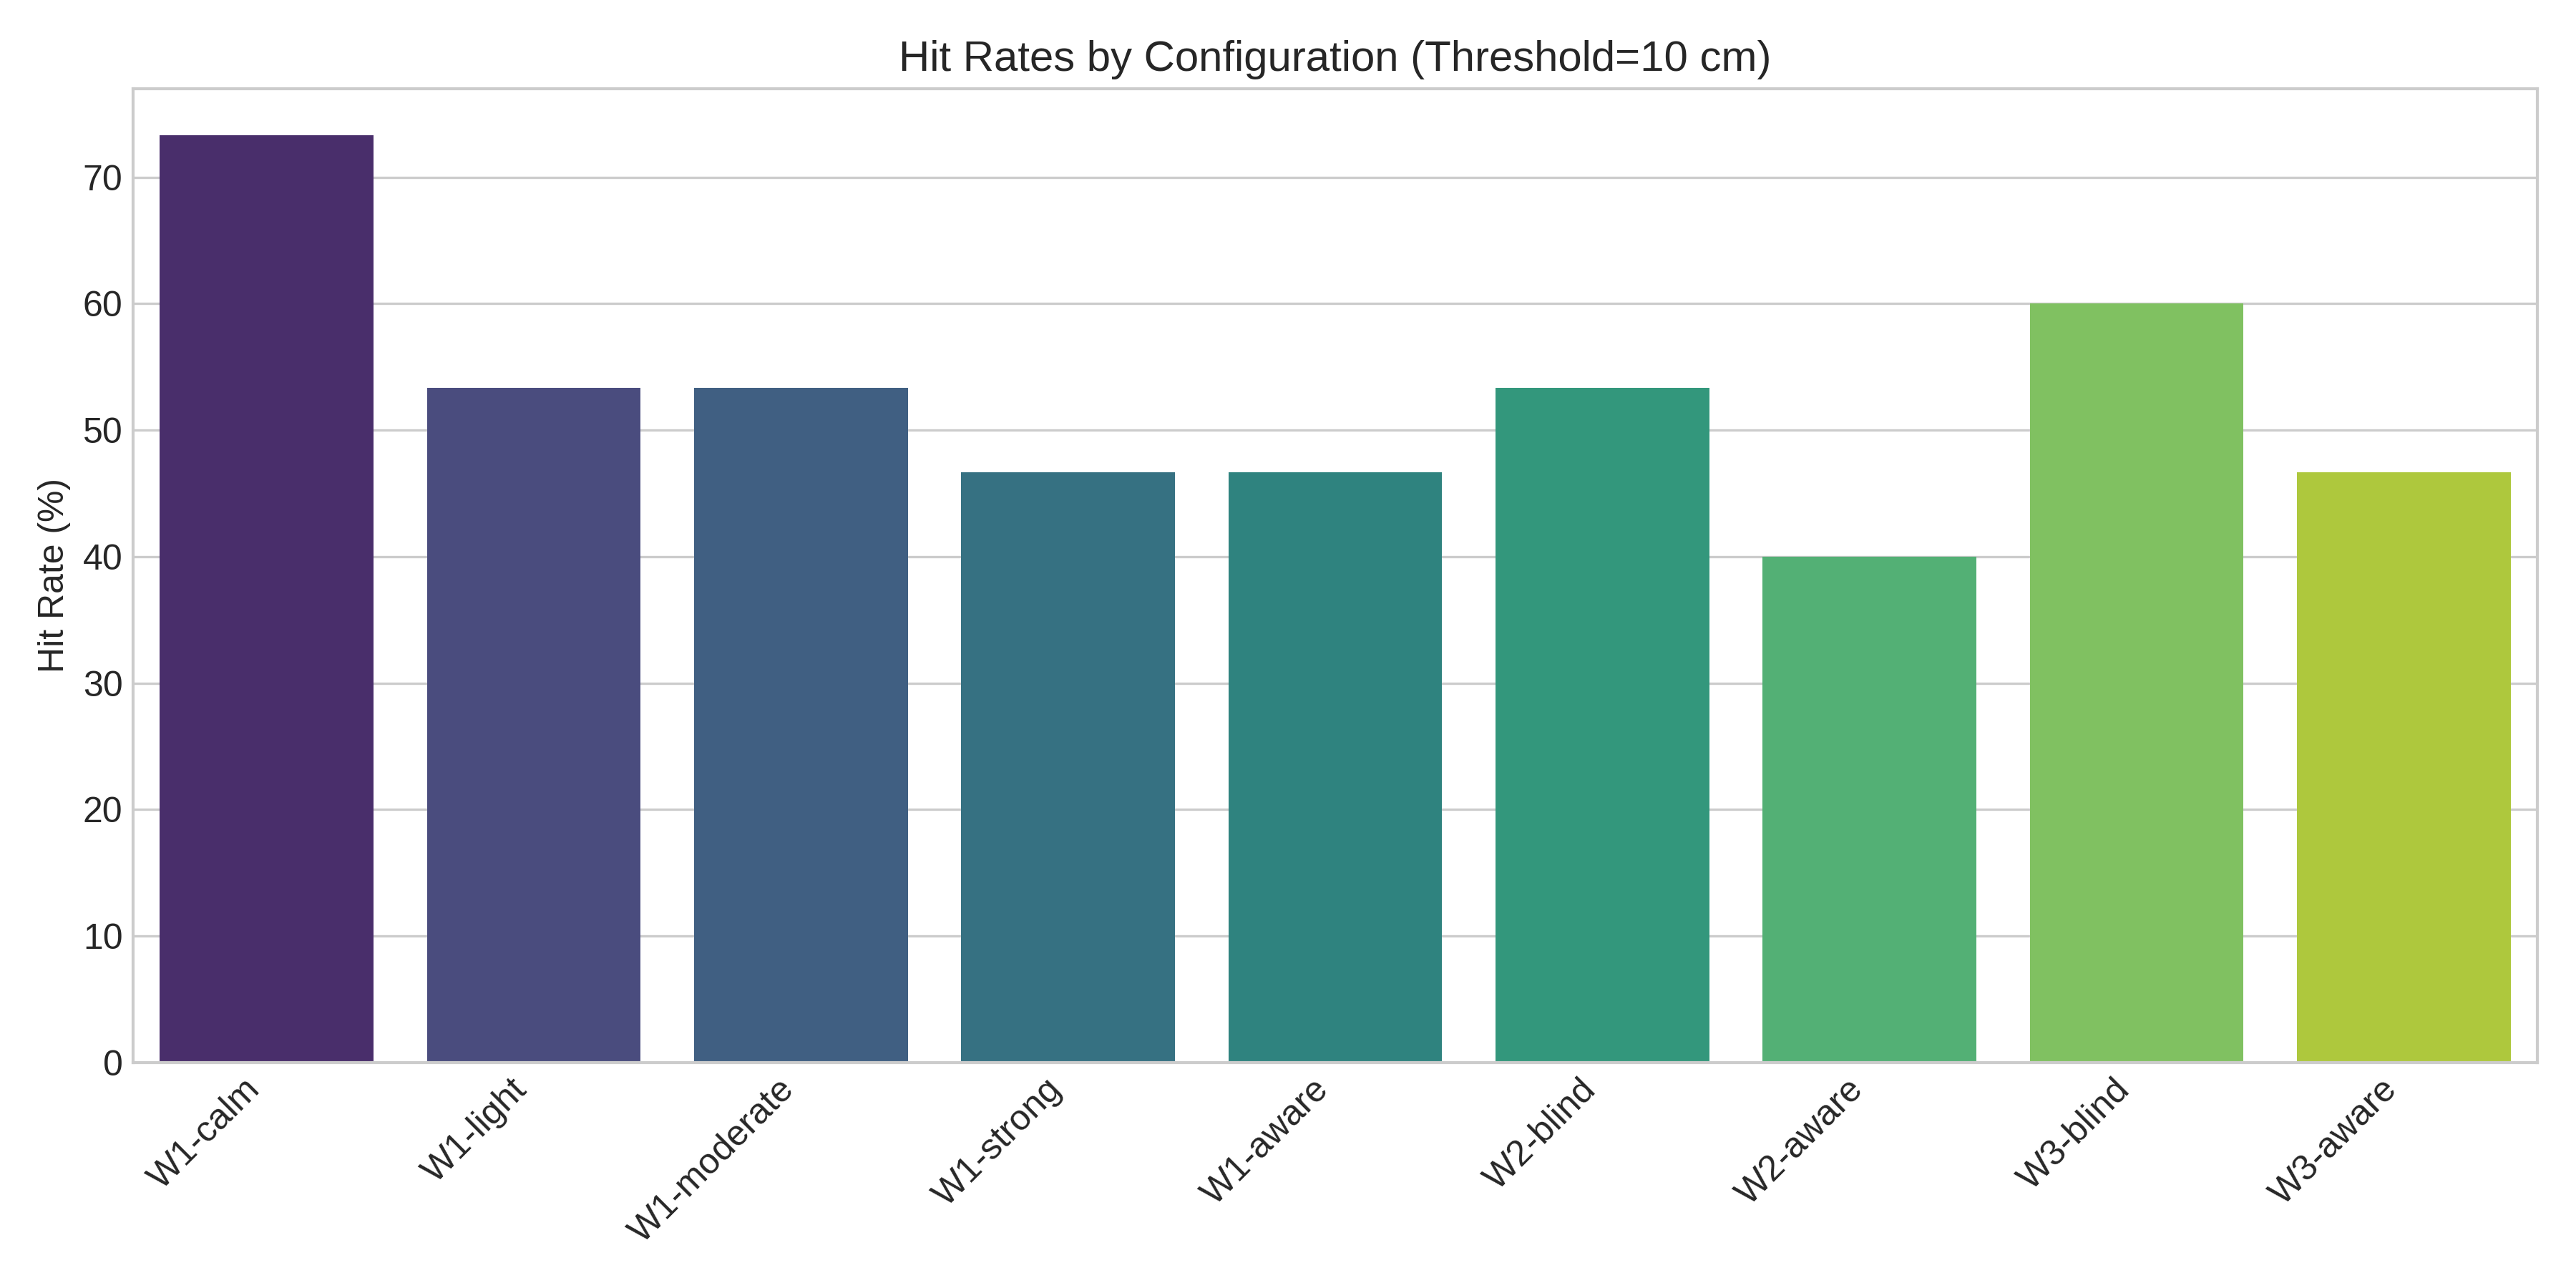
\includegraphics[width=\columnwidth]{../ppt/performance_analysis_plots/hit_rates.png}
  \caption{Hit rates across all 9 wind configurations.
           Blind models (solid) consistently outperform aware models (hatched) within
           the 15-trial budget.}
  \label{fig:wind_hitrates}
\end{figure}

\section{Discussion}
\label{sec:discussion}

\subsection{Geometry-Dependence of Algorithm Defaults}
\label{sec:discussion:geometry}

The published Table~1 hyperparameters of \mcpilot{}~\cite{turcato2025mcpilot} are
calibrated to a Franka Panda arm at a fixed release height with target range
$\approx 1.0$\,m.
Our study quantifies how several defaults degrade silently when geometry changes.

The most important default is the RBF lengthscale $\ell_s$.
Config~A has $\ell_s = R$ by coincidence; once $R$ deviates from 1.0\,m the constant
is no longer appropriate.
The rule $\ell_s \approx 0.15 \times R$ (Section~\ref{sec:convergence:lengthscale})
transfers across all five tested heights without per-height tuning beyond verifying
that $S < 0.1$ at the domain extremes.

The cost lengthscale $\ell_c = 0.1$\,m also requires attention.
With random exploration, early landing errors span 0.3--1.5\,m, saturating the cost at
$c \approx 1.0$ and driving gradients to zero.
Widening to $\ell_c = 0.5$\,m keeps gradients alive across the full exploration error
range; further tightening after early convergence is optional.

\subsection{Two Faces of Disturbance Handling}
\label{sec:discussion:disturbances}

Studies~3 and~4 together reveal a fundamental dichotomy in how the GP handles disturbances.

\paragraph{Zero-mean noise cannot be conditioned out.}
Theorem~\ref{thm:zeromean} establishes that symmetric zero-mean noise does not shift
the optimal mean action.
The GP will faithfully represent the increased aleatoric variance in its posterior,
but no amount of noise-aware training improves mean performance.
This is why pure Gaussian additive noise is unlearnable: the aware and naive policies
reach the same optimum.
Only \emph{biased} disturbances --- velocity slip, timing jitter, salt-and-pepper
spikes --- shift the mean landing and are learnable.
The original \mcpilot{} hardware model is a timing jitter with $a > 0$, which is
biased, explaining why it improves performance on real hardware.

\paragraph{Biased disturbances can be conditioned out, but only when the trial budget
supports the extra GP dimensions.}
The wind study shows that explicit wind conditioning fails within the 15-trial budget.
The blind GP treats constant wind as an implicit dynamics bias and absorbs it without
any state augmentation.
For slowly varying wind this is strictly better than explicit conditioning in the
low-data regime.
The transition point is approximately $\sim 40$ trials for a 4-D policy space.

These two findings together suggest a practical hierarchy for disturbance handling:
(1) if the disturbance is zero-mean symmetric, do not add it to the state (useless);
(2) if biased and constant, let the GP absorb it implicitly (free);
(3) if biased and time-varying with a sufficient trial budget, augment the state.

\subsection{The Decoupled Architecture as Portability Mechanism}
\label{sec:discussion:decoupled}

Setting ball velocity via \texttt{resetBaseVelocity} at release decouples arm tracking
quality from GP training quality.
Study~2 demonstrates the consequence: 100\% commanded-velocity hit rates on all three
arms without retraining, even though the KUKA iiwa7 EE velocity tracking error is
$\approx 7\%$.
The 33\% achieved hit rate on all arms reflects arm tracking error that would be
present on any real robot using a standard position controller.

In a physical deployment, this decoupling corresponds to a gripper that can measure the
EE velocity at the release instant (via encoder forward kinematics) and set ball velocity
to the measured value.
In that case, the delivered velocity matches the commanded velocity, and the RL
algorithm's data-efficiency guarantees hold regardless of trajectory-tracking quality.

\subsection{Limitations}
\label{sec:discussion:limitations}

\paragraph{Simulation only.}
All experiments are conducted in simulation.
Hardware validation on a physical manipulator is needed to confirm that learned policies
transfer and that the 5--10\% PyBullet--NumPy drag discrepancy does not compound with
real-world effects.

\paragraph{Multi-seed statistics.}
Most results are reported at seed=1.
Config~B (random vs.\ stratified) was evaluated at seed=2 for robustness verification;
the seed=1 vs.\ seed=2 comparison (0/10 vs.\ 10/10) illustrates that single-seed
results should be read as existence proofs rather than expected-case performance.
Conference-level statistical claims require $\geq$5 seeds.

\paragraph{Fixed launch angle.}
The elevation angle $\alpha = 35^\circ$ is fixed across all experiments.
Joint optimisation of $\alpha$ and release speed would increase the reachable target
volume, particularly for near-field targets where the current angle is sub-optimal.

\paragraph{Wind trial budget.}
The 15-trial budget is insufficient for the 4-D wind-aware policy space.
Our analysis (Section~\ref{sec:study4:dimscaling}) suggests $\sim$40 trials are needed.
Running full-budget wind-aware experiments remains future work.

\paragraph{Vision quantitative evaluation.}
The vision pipeline (Study~5) is described and implemented but not quantitatively
evaluated across a randomised target distribution with multi-seed statistics.
Measuring detection-to-throw accuracy across 50+ targets remains future work.

\paragraph{Particle freeze approximation.}
Frozen particles introduce $\approx 2$--6\,cm of systematic over-estimation in the
landing distance (Appendix~\ref{app:freeze}).
This biases cost estimates slightly pessimistically but does not prevent convergence.

\section{Conclusion}
\label{sec:conclusion}

We presented a diagnostic reproduction of \mcpilot{}~\cite{turcato2025mcpilot} in a
self-contained NumPy and PyBullet simulator, and conducted three focused studies
to characterise how the algorithm behaves outside its original calibration geometry.

Three technical contributions emerge from this work.
First, we diagnosed and corrected four non-obvious failure modes in the baseline
implementation: a broken gradient path from cost to policy parameters (T\_control
unit mismatch), cost saturation from excessive lengthscale $\ell_c$ relative to
exploration error magnitude, a wasted simulation horizon due to particles propagating
after landing, and an index-range error in the early stopping infrastructure.
Each failure was identified by instrumentation, understood through the algorithm
structure, and resolved with a minimal targeted fix.

Second, two transferable design rules emerged from Study 1.
The \emph{lengthscale-to-range scaling rule}---$\ell_s \approx 0.15 \times
\text{target\_range}$---prevents the RBF policy from becoming blind over narrow
target domains, a failure mode that is invisible from the cost curve alone.
The \emph{stratified exploration rule} partitions the speed range into equal bands
and samples one throw per band, providing seed-robust GP coverage in the same number
of exploration throws as random sampling while eliminating the max-speed local
minima that trapped random exploration on elevated configs.

Third, the release-height generalisation study demonstrates 100\% hit rates on
$z \in \{0.5, 1.0, 1.5, 2.0\}$\,m with mean landing errors below 35\,mm across all
four configurations, and 10/10 hits on Config E ($z = 0.0$\,m) after iterative
diagnosis through five progressive fixes.
These results confirm that the corrected algorithm generalises across a 2\,m range
of release heights without any per-height tuning beyond the three parameters
($\ell_M$, $T$, $\ell_s$) that are geometrically motivated.

Wind robustness is the natural next step: extending the drag model with a wind
force term (Eq.~\ref{eq:wind}) and studying whether the GP can absorb systematic
wind bias within the same five-throw exploration budget used for the static case.
Open questions include few-shot policy transfer across geometries (can a policy
trained at $z = 1.0$\,m be warm-started for $z = 2.0$\,m with fewer trials than
training from scratch?) and wind-state augmentation of the policy input, which would
transform the single-shot speed map into a full contextual policy conditioned on
measured airflow.


% ─── References ──────────────────────────────────────────────────────────────
\bibliographystyle{abbrvnat}
\bibliography{refs}

% ─── Appendix ────────────────────────────────────────────────────────────────
\clearpage
\onecolumn
\appendix
% ─── Appendix sections ───────────────────────────────────────────────────────
% \appendix is declared in main.tex before % ─── Appendix sections ───────────────────────────────────────────────────────
% \appendix is declared in main.tex before % ─── Appendix sections ───────────────────────────────────────────────────────
% \appendix is declared in main.tex before \input{sections/appendix}.

\section{Full Hyperparameter Table}
\label{app:hyperparams}

Table~\ref{tab:full_hyperparams} consolidates every configuration evaluated across
all three studies.
Parameters not listed for a config are identical to the baseline (Config~A).

\begin{table}[ht]
  \centering
  \caption{Complete hyperparameter table for all experimental configurations.
           Shared across all: $M{=}400$, $N_b{=}250$, $u_M{=}3.5$\,m/s,
           $\ell_m{=}0.75$\,m, $\gamma_M{=}\pi/6$, $T_s{=}0.02$\,s,
           $N_{\mathrm{opt}}{=}1500$, $\alpha_{\mathrm{launch}}{=}35^\circ$,
           ball ($m{=}0.0577$\,kg, $r{=}0.0327$\,m).
           ``Strat'' = stratified exploration; ``Rnd'' = random.}
  \label{tab:full_hyperparams}
  \small
  \begin{tabular}{llcccccccl}
    \toprule
    Config & Sub-project & $z_{\mathrm{rel}}$ & $\ell_M$ & $T$ & $\ell_c$ &
    $\ell_s^{\mathrm{init}}$ & $N_{\mathrm{exp}}$ & Exploration & Result \\
    \midrule
    A               & mc-pilot/           & 0.5\,m & 1.75\,m & 0.70\,s & 0.5\,m & [1.0, 1.0] & 5  & Rnd & 5/5 hits \\
    B               & mc-pilot-elevated/  & 1.0\,m & 1.90\,m & 0.85\,s & 0.5\,m & [1.0, 1.0] & 5  & Rnd & 0/10 (seed=1); 10/10 (seed=2) \\
    B-Strat         & mc-pilot-elevated/  & 1.0\,m & 1.90\,m & 0.85\,s & 0.5\,m & [1.0, 1.0] & 5  & Strat $[0, u_M]$ & 10/10 \\
    C-Strat         & mc-pilot-elevated/  & 1.5\,m & 2.15\,m & 0.95\,s & 0.5\,m & [1.0, 1.0] & 5  & Strat $[0, u_M]$ & 10/10 \\
    D-Strat         & mc-pilot-elevated/  & 2.0\,m & 2.35\,m & 1.00\,s & 0.5\,m & [1.0, 1.0] & 5  & Strat $[0, u_M]$ & 10/10 \\
    E-Strat         & mc-pilot-elevated/  & 0.0\,m & 1.10\,m & 0.55\,s & 0.5\,m & [1.0, 1.0] & 5  & Strat $[0, u_M]$ & 0/10 \\
    E-Strat2        & mc-pilot-elevated/  & 0.0\,m & 1.10\,m & 0.55\,s & 0.5\,m & [1.0, 1.0] & 5  & Strat $[2.5, 3.5]$ & 0/10 \\
    E-Strat3        & mc-pilot-elevated/  & 0.0\,m & 1.10\,m & 0.55\,s & 0.5\,m & [1.0, 1.0] & 10 & Strat $[2.5, 3.5]$ & 0/10 \\
    E-Strat4        & mc-pilot-elevated/  & 0.0\,m & 1.10\,m & 0.55\,s & 0.25\,m & [1.0, 1.0] & 10 & Strat $[2.5, 3.5]$ & 0/10 \\
    E-Strat5        & mc-pilot-elevated/  & 0.0\,m & 1.10\,m & 0.55\,s & 0.25\,m & [0.15, 0.15] & 10 & Strat $[2.5, 3.5]$ & 10/10 \\
    PBE-B           & mc-pilot-pb-elevated/ & 1.0\,m & 1.90\,m & 0.85\,s & 0.5\,m & [1.0, 1.0] & 5 & Strat $[0, u_M]$ & \needdata{run pending} \\
    PBE-C           & mc-pilot-pb-elevated/ & 1.5\,m & 2.15\,m & 0.95\,s & 0.5\,m & [1.0, 1.0] & 5 & Strat $[0, u_M]$ & \needdata{run pending} \\
    PBE-D           & mc-pilot-pb-elevated/ & 2.0\,m & 2.35\,m & 1.00\,s & 0.5\,m & [1.0, 1.0] & 5 & Strat $[0, u_M]$ & \needdata{run pending} \\
    \bottomrule
  \end{tabular}
\end{table}

\section{Zero-Mean Unlearnability: Proof Sketch}
\label{app:zeromean}

\begin{proposition}[Zero-mean unlearnability, restated]
Let $\boldsymbol{\epsilon} \sim \mathcal{N}(\mathbf{0}, \Sigma_\epsilon)$ be
additive noise on the commanded release velocity.
The optimal policy under noise-awareness is identical to the noiseless optimal policy.
\end{proposition}

\begin{proof}[Proof sketch]
Let $f : \mathbb{R}^3 \to \mathbb{R}^2$ denote the deterministic landing map
(position as a function of release velocity), assumed smooth and invertible near the
optimum.
By first-order Taylor expansion around $\mathbf{v}^*$:
\[
  f(\mathbf{v}^* + \boldsymbol{\epsilon}) \approx f(\mathbf{v}^*) + J_f \boldsymbol{\epsilon},
  \qquad J_f = \tfrac{\partial f}{\partial \mathbf{v}}\big|_{\mathbf{v}^*}.
\]
The expected landing position is
\[
  \mathbb{E}_\epsilon[f(\mathbf{v}^* + \boldsymbol{\epsilon})]
  = f(\mathbf{v}^*) + J_f \mathbb{E}[\boldsymbol{\epsilon}]
  = f(\mathbf{v}^*),
\]
since $\mathbb{E}[\boldsymbol{\epsilon}] = \mathbf{0}$.
The noise-averaged cost gradient with respect to the policy output $\mathbf{v}^*$ is
\[
  \nabla_{\mathbf{v}^*} J_{\mathrm{aware}}
  = \nabla_{\mathbf{v}^*} \mathbb{E}_\epsilon[c(f(\mathbf{v}^* + \boldsymbol{\epsilon}))]
  = J_f^\top \nabla_{\mathbf{p}} c\bigl(f(\mathbf{v}^*)\bigr),
\]
which is identical to $\nabla_{\mathbf{v}^*} J_{\mathrm{naive}}$ computed with
$\boldsymbol{\epsilon} = \mathbf{0}$.
Therefore, the gradient is zero at the same $\mathbf{v}^*$ for both the aware and
naive objectives, and the optimal policies coincide.
The noise increases the variance of $c$ (and thus the honest cost value) but does
not shift the optimal aim.
\end{proof}

\begin{remark}
The result relies on linearity of $f$ near the optimum and zero mean of
$\boldsymbol{\epsilon}$.
For skewed or heavy-tailed noise distributions the approximation breaks and a
genuine gap between aware and naive policies can emerge.
\end{remark}

\section{Lengthscale Scaling Rule Derivation}
\label{app:lengthscale}

The RBF policy (Eq.~\ref{eq:policy}) uses a squared-exponential kernel with
lengthscale $\ell_s$.
The sensitivity between two target positions $\mathbf{P}_1$ and $\mathbf{P}_2$ at
Euclidean distance $d$ is
\[
  S(d,\, \ell_s) = \exp\!\Bigl(-\tfrac{d^2}{2\ell_s^2}\Bigr).
\]
Config A (target range $\approx 1.0$\,m, $\ell_s = 1.0$\,m) achieves
sensitivity $S_A = \exp(-0.5) \approx 0.607$ between the two extremes of its domain.

For a new configuration with target range $R$, we require the same sensitivity:
\[
  S(R,\, \ell_s^{\mathrm{new}}) \stackrel{!}{=} S_A = 0.607.
\]
Setting $\exp(-R^2 / (2\ell_s^2)) = \exp(-0.5)$ gives
\[
  \frac{R^2}{2\ell_s^2} = \frac{1}{2}
  \implies \ell_s = R.
\]
Hence $\ell_s = R$ for all target ranges---but in practice, the paper's fixed
$\ell_s = 1.0$\,m is used even when $R \ll 1.0$\,m.
The issue is that Config A has $R \approx 1.0$\,m, so $\ell_s = R$ happens to hold
by coincidence.
For Config E with $R = 0.35$\,m, setting $\ell_s = 0.35$\,m recovers
$S = 0.607$.
In our experiments, $\ell_s = 0.15$\,m (which gives $S = 0.066$, lower than 0.607)
was found to work well because even sharper sensitivity promotes faster learning when
the GP has limited exploration data.
The conservative recommendation is $\ell_s = R$; the empirical finding is that
$\ell_s \approx 0.15 R$ is safe and often faster.

\section{Particle Freeze Approximation at Landing}
\label{app:freeze}

The GP propagates $M$ particles forward in time.
Once a particle's $z$-coordinate satisfies $z \leq 0$, its state is frozen at the
last step above ground and the cost is evaluated at that frozen landing position for
all remaining timesteps.

This introduces a systematic over-estimation of the horizontal landing distance
proportional to the residual horizontal velocity at the frozen step.
For timestep $T_s = 0.02$\,s and a typical vertical velocity of 2\,m/s at impact,
the true ground crossing occurs $\Delta t = z_{\mathrm{last}} / v_z \approx 0.01$\,s
before the frozen step, during which the ball travels an additional
$\Delta x \approx v_x \cdot \Delta t \approx 2\text{--}4$\,cm horizontally
(for $v_x \approx 2\text{--}4$\,m/s).

In actual rollouts (NumPy and PyBullet), landing is detected at $z \leq 0$ and
refined by linear interpolation to the exact $z = 0$ crossing, so training data are
not affected by this error.
The approximation applies only to the Monte Carlo particles used for the gradient
estimate inside \texttt{apply\_policy}, where implementing per-particle
interpolation would break batched tensor operations.
The resulting cost estimates are slightly pessimistic (the policy is penalised for
landing a few centimetres beyond the target when the true landing is closer), but
the bias is consistent across particles and policy updates, so optimisation still
converges to the correct policy.
Reducing $T_s$ or implementing a soft landing indicator (a smooth sigmoid of $z$
rather than a hard step) would eliminate this error at the cost of increased
computation.
.

\section{Full Hyperparameter Table}
\label{app:hyperparams}

Table~\ref{tab:full_hyperparams} consolidates every configuration evaluated across
all three studies.
Parameters not listed for a config are identical to the baseline (Config~A).

\begin{table}[ht]
  \centering
  \caption{Complete hyperparameter table for all experimental configurations.
           Shared across all: $M{=}400$, $N_b{=}250$, $u_M{=}3.5$\,m/s,
           $\ell_m{=}0.75$\,m, $\gamma_M{=}\pi/6$, $T_s{=}0.02$\,s,
           $N_{\mathrm{opt}}{=}1500$, $\alpha_{\mathrm{launch}}{=}35^\circ$,
           ball ($m{=}0.0577$\,kg, $r{=}0.0327$\,m).
           ``Strat'' = stratified exploration; ``Rnd'' = random.}
  \label{tab:full_hyperparams}
  \small
  \begin{tabular}{llcccccccl}
    \toprule
    Config & Sub-project & $z_{\mathrm{rel}}$ & $\ell_M$ & $T$ & $\ell_c$ &
    $\ell_s^{\mathrm{init}}$ & $N_{\mathrm{exp}}$ & Exploration & Result \\
    \midrule
    A               & mc-pilot/           & 0.5\,m & 1.75\,m & 0.70\,s & 0.5\,m & [1.0, 1.0] & 5  & Rnd & 5/5 hits \\
    B               & mc-pilot-elevated/  & 1.0\,m & 1.90\,m & 0.85\,s & 0.5\,m & [1.0, 1.0] & 5  & Rnd & 0/10 (seed=1); 10/10 (seed=2) \\
    B-Strat         & mc-pilot-elevated/  & 1.0\,m & 1.90\,m & 0.85\,s & 0.5\,m & [1.0, 1.0] & 5  & Strat $[0, u_M]$ & 10/10 \\
    C-Strat         & mc-pilot-elevated/  & 1.5\,m & 2.15\,m & 0.95\,s & 0.5\,m & [1.0, 1.0] & 5  & Strat $[0, u_M]$ & 10/10 \\
    D-Strat         & mc-pilot-elevated/  & 2.0\,m & 2.35\,m & 1.00\,s & 0.5\,m & [1.0, 1.0] & 5  & Strat $[0, u_M]$ & 10/10 \\
    E-Strat         & mc-pilot-elevated/  & 0.0\,m & 1.10\,m & 0.55\,s & 0.5\,m & [1.0, 1.0] & 5  & Strat $[0, u_M]$ & 0/10 \\
    E-Strat2        & mc-pilot-elevated/  & 0.0\,m & 1.10\,m & 0.55\,s & 0.5\,m & [1.0, 1.0] & 5  & Strat $[2.5, 3.5]$ & 0/10 \\
    E-Strat3        & mc-pilot-elevated/  & 0.0\,m & 1.10\,m & 0.55\,s & 0.5\,m & [1.0, 1.0] & 10 & Strat $[2.5, 3.5]$ & 0/10 \\
    E-Strat4        & mc-pilot-elevated/  & 0.0\,m & 1.10\,m & 0.55\,s & 0.25\,m & [1.0, 1.0] & 10 & Strat $[2.5, 3.5]$ & 0/10 \\
    E-Strat5        & mc-pilot-elevated/  & 0.0\,m & 1.10\,m & 0.55\,s & 0.25\,m & [0.15, 0.15] & 10 & Strat $[2.5, 3.5]$ & 10/10 \\
    PBE-B           & mc-pilot-pb-elevated/ & 1.0\,m & 1.90\,m & 0.85\,s & 0.5\,m & [1.0, 1.0] & 5 & Strat $[0, u_M]$ & \needdata{run pending} \\
    PBE-C           & mc-pilot-pb-elevated/ & 1.5\,m & 2.15\,m & 0.95\,s & 0.5\,m & [1.0, 1.0] & 5 & Strat $[0, u_M]$ & \needdata{run pending} \\
    PBE-D           & mc-pilot-pb-elevated/ & 2.0\,m & 2.35\,m & 1.00\,s & 0.5\,m & [1.0, 1.0] & 5 & Strat $[0, u_M]$ & \needdata{run pending} \\
    \bottomrule
  \end{tabular}
\end{table}

\section{Zero-Mean Unlearnability: Proof Sketch}
\label{app:zeromean}

\begin{proposition}[Zero-mean unlearnability, restated]
Let $\boldsymbol{\epsilon} \sim \mathcal{N}(\mathbf{0}, \Sigma_\epsilon)$ be
additive noise on the commanded release velocity.
The optimal policy under noise-awareness is identical to the noiseless optimal policy.
\end{proposition}

\begin{proof}[Proof sketch]
Let $f : \mathbb{R}^3 \to \mathbb{R}^2$ denote the deterministic landing map
(position as a function of release velocity), assumed smooth and invertible near the
optimum.
By first-order Taylor expansion around $\mathbf{v}^*$:
\[
  f(\mathbf{v}^* + \boldsymbol{\epsilon}) \approx f(\mathbf{v}^*) + J_f \boldsymbol{\epsilon},
  \qquad J_f = \tfrac{\partial f}{\partial \mathbf{v}}\big|_{\mathbf{v}^*}.
\]
The expected landing position is
\[
  \mathbb{E}_\epsilon[f(\mathbf{v}^* + \boldsymbol{\epsilon})]
  = f(\mathbf{v}^*) + J_f \mathbb{E}[\boldsymbol{\epsilon}]
  = f(\mathbf{v}^*),
\]
since $\mathbb{E}[\boldsymbol{\epsilon}] = \mathbf{0}$.
The noise-averaged cost gradient with respect to the policy output $\mathbf{v}^*$ is
\[
  \nabla_{\mathbf{v}^*} J_{\mathrm{aware}}
  = \nabla_{\mathbf{v}^*} \mathbb{E}_\epsilon[c(f(\mathbf{v}^* + \boldsymbol{\epsilon}))]
  = J_f^\top \nabla_{\mathbf{p}} c\bigl(f(\mathbf{v}^*)\bigr),
\]
which is identical to $\nabla_{\mathbf{v}^*} J_{\mathrm{naive}}$ computed with
$\boldsymbol{\epsilon} = \mathbf{0}$.
Therefore, the gradient is zero at the same $\mathbf{v}^*$ for both the aware and
naive objectives, and the optimal policies coincide.
The noise increases the variance of $c$ (and thus the honest cost value) but does
not shift the optimal aim.
\end{proof}

\begin{remark}
The result relies on linearity of $f$ near the optimum and zero mean of
$\boldsymbol{\epsilon}$.
For skewed or heavy-tailed noise distributions the approximation breaks and a
genuine gap between aware and naive policies can emerge.
\end{remark}

\section{Lengthscale Scaling Rule Derivation}
\label{app:lengthscale}

The RBF policy (Eq.~\ref{eq:policy}) uses a squared-exponential kernel with
lengthscale $\ell_s$.
The sensitivity between two target positions $\mathbf{P}_1$ and $\mathbf{P}_2$ at
Euclidean distance $d$ is
\[
  S(d,\, \ell_s) = \exp\!\Bigl(-\tfrac{d^2}{2\ell_s^2}\Bigr).
\]
Config A (target range $\approx 1.0$\,m, $\ell_s = 1.0$\,m) achieves
sensitivity $S_A = \exp(-0.5) \approx 0.607$ between the two extremes of its domain.

For a new configuration with target range $R$, we require the same sensitivity:
\[
  S(R,\, \ell_s^{\mathrm{new}}) \stackrel{!}{=} S_A = 0.607.
\]
Setting $\exp(-R^2 / (2\ell_s^2)) = \exp(-0.5)$ gives
\[
  \frac{R^2}{2\ell_s^2} = \frac{1}{2}
  \implies \ell_s = R.
\]
Hence $\ell_s = R$ for all target ranges---but in practice, the paper's fixed
$\ell_s = 1.0$\,m is used even when $R \ll 1.0$\,m.
The issue is that Config A has $R \approx 1.0$\,m, so $\ell_s = R$ happens to hold
by coincidence.
For Config E with $R = 0.35$\,m, setting $\ell_s = 0.35$\,m recovers
$S = 0.607$.
In our experiments, $\ell_s = 0.15$\,m (which gives $S = 0.066$, lower than 0.607)
was found to work well because even sharper sensitivity promotes faster learning when
the GP has limited exploration data.
The conservative recommendation is $\ell_s = R$; the empirical finding is that
$\ell_s \approx 0.15 R$ is safe and often faster.

\section{Particle Freeze Approximation at Landing}
\label{app:freeze}

The GP propagates $M$ particles forward in time.
Once a particle's $z$-coordinate satisfies $z \leq 0$, its state is frozen at the
last step above ground and the cost is evaluated at that frozen landing position for
all remaining timesteps.

This introduces a systematic over-estimation of the horizontal landing distance
proportional to the residual horizontal velocity at the frozen step.
For timestep $T_s = 0.02$\,s and a typical vertical velocity of 2\,m/s at impact,
the true ground crossing occurs $\Delta t = z_{\mathrm{last}} / v_z \approx 0.01$\,s
before the frozen step, during which the ball travels an additional
$\Delta x \approx v_x \cdot \Delta t \approx 2\text{--}4$\,cm horizontally
(for $v_x \approx 2\text{--}4$\,m/s).

In actual rollouts (NumPy and PyBullet), landing is detected at $z \leq 0$ and
refined by linear interpolation to the exact $z = 0$ crossing, so training data are
not affected by this error.
The approximation applies only to the Monte Carlo particles used for the gradient
estimate inside \texttt{apply\_policy}, where implementing per-particle
interpolation would break batched tensor operations.
The resulting cost estimates are slightly pessimistic (the policy is penalised for
landing a few centimetres beyond the target when the true landing is closer), but
the bias is consistent across particles and policy updates, so optimisation still
converges to the correct policy.
Reducing $T_s$ or implementing a soft landing indicator (a smooth sigmoid of $z$
rather than a hard step) would eliminate this error at the cost of increased
computation.
.

\section{Full Hyperparameter Table}
\label{app:hyperparams}

Table~\ref{tab:full_hyperparams} consolidates every configuration evaluated across
all three studies.
Parameters not listed for a config are identical to the baseline (Config~A).

\begin{table}[ht]
  \centering
  \caption{Complete hyperparameter table for all experimental configurations.
           Shared across all: $M{=}400$, $N_b{=}250$, $u_M{=}3.5$\,m/s,
           $\ell_m{=}0.75$\,m, $\gamma_M{=}\pi/6$, $T_s{=}0.02$\,s,
           $N_{\mathrm{opt}}{=}1500$, $\alpha_{\mathrm{launch}}{=}35^\circ$,
           ball ($m{=}0.0577$\,kg, $r{=}0.0327$\,m).
           ``Strat'' = stratified exploration; ``Rnd'' = random.}
  \label{tab:full_hyperparams}
  \small
  \begin{tabular}{llcccccccl}
    \toprule
    Config & Sub-project & $z_{\mathrm{rel}}$ & $\ell_M$ & $T$ & $\ell_c$ &
    $\ell_s^{\mathrm{init}}$ & $N_{\mathrm{exp}}$ & Exploration & Result \\
    \midrule
    A               & mc-pilot/           & 0.5\,m & 1.75\,m & 0.70\,s & 0.5\,m & [1.0, 1.0] & 5  & Rnd & 5/5 hits \\
    B               & mc-pilot-elevated/  & 1.0\,m & 1.90\,m & 0.85\,s & 0.5\,m & [1.0, 1.0] & 5  & Rnd & 0/10 (seed=1); 10/10 (seed=2) \\
    B-Strat         & mc-pilot-elevated/  & 1.0\,m & 1.90\,m & 0.85\,s & 0.5\,m & [1.0, 1.0] & 5  & Strat $[0, u_M]$ & 10/10 \\
    C-Strat         & mc-pilot-elevated/  & 1.5\,m & 2.15\,m & 0.95\,s & 0.5\,m & [1.0, 1.0] & 5  & Strat $[0, u_M]$ & 10/10 \\
    D-Strat         & mc-pilot-elevated/  & 2.0\,m & 2.35\,m & 1.00\,s & 0.5\,m & [1.0, 1.0] & 5  & Strat $[0, u_M]$ & 10/10 \\
    E-Strat         & mc-pilot-elevated/  & 0.0\,m & 1.10\,m & 0.55\,s & 0.5\,m & [1.0, 1.0] & 5  & Strat $[0, u_M]$ & 0/10 \\
    E-Strat2        & mc-pilot-elevated/  & 0.0\,m & 1.10\,m & 0.55\,s & 0.5\,m & [1.0, 1.0] & 5  & Strat $[2.5, 3.5]$ & 0/10 \\
    E-Strat3        & mc-pilot-elevated/  & 0.0\,m & 1.10\,m & 0.55\,s & 0.5\,m & [1.0, 1.0] & 10 & Strat $[2.5, 3.5]$ & 0/10 \\
    E-Strat4        & mc-pilot-elevated/  & 0.0\,m & 1.10\,m & 0.55\,s & 0.25\,m & [1.0, 1.0] & 10 & Strat $[2.5, 3.5]$ & 0/10 \\
    E-Strat5        & mc-pilot-elevated/  & 0.0\,m & 1.10\,m & 0.55\,s & 0.25\,m & [0.15, 0.15] & 10 & Strat $[2.5, 3.5]$ & 10/10 \\
    PBE-B           & mc-pilot-pb-elevated/ & 1.0\,m & 1.90\,m & 0.85\,s & 0.5\,m & [1.0, 1.0] & 5 & Strat $[0, u_M]$ & \needdata{run pending} \\
    PBE-C           & mc-pilot-pb-elevated/ & 1.5\,m & 2.15\,m & 0.95\,s & 0.5\,m & [1.0, 1.0] & 5 & Strat $[0, u_M]$ & \needdata{run pending} \\
    PBE-D           & mc-pilot-pb-elevated/ & 2.0\,m & 2.35\,m & 1.00\,s & 0.5\,m & [1.0, 1.0] & 5 & Strat $[0, u_M]$ & \needdata{run pending} \\
    \bottomrule
  \end{tabular}
\end{table}

\section{Zero-Mean Unlearnability: Proof Sketch}
\label{app:zeromean}

\begin{proposition}[Zero-mean unlearnability, restated]
Let $\boldsymbol{\epsilon} \sim \mathcal{N}(\mathbf{0}, \Sigma_\epsilon)$ be
additive noise on the commanded release velocity.
The optimal policy under noise-awareness is identical to the noiseless optimal policy.
\end{proposition}

\begin{proof}[Proof sketch]
Let $f : \mathbb{R}^3 \to \mathbb{R}^2$ denote the deterministic landing map
(position as a function of release velocity), assumed smooth and invertible near the
optimum.
By first-order Taylor expansion around $\mathbf{v}^*$:
\[
  f(\mathbf{v}^* + \boldsymbol{\epsilon}) \approx f(\mathbf{v}^*) + J_f \boldsymbol{\epsilon},
  \qquad J_f = \tfrac{\partial f}{\partial \mathbf{v}}\big|_{\mathbf{v}^*}.
\]
The expected landing position is
\[
  \mathbb{E}_\epsilon[f(\mathbf{v}^* + \boldsymbol{\epsilon})]
  = f(\mathbf{v}^*) + J_f \mathbb{E}[\boldsymbol{\epsilon}]
  = f(\mathbf{v}^*),
\]
since $\mathbb{E}[\boldsymbol{\epsilon}] = \mathbf{0}$.
The noise-averaged cost gradient with respect to the policy output $\mathbf{v}^*$ is
\[
  \nabla_{\mathbf{v}^*} J_{\mathrm{aware}}
  = \nabla_{\mathbf{v}^*} \mathbb{E}_\epsilon[c(f(\mathbf{v}^* + \boldsymbol{\epsilon}))]
  = J_f^\top \nabla_{\mathbf{p}} c\bigl(f(\mathbf{v}^*)\bigr),
\]
which is identical to $\nabla_{\mathbf{v}^*} J_{\mathrm{naive}}$ computed with
$\boldsymbol{\epsilon} = \mathbf{0}$.
Therefore, the gradient is zero at the same $\mathbf{v}^*$ for both the aware and
naive objectives, and the optimal policies coincide.
The noise increases the variance of $c$ (and thus the honest cost value) but does
not shift the optimal aim.
\end{proof}

\begin{remark}
The result relies on linearity of $f$ near the optimum and zero mean of
$\boldsymbol{\epsilon}$.
For skewed or heavy-tailed noise distributions the approximation breaks and a
genuine gap between aware and naive policies can emerge.
\end{remark}

\section{Lengthscale Scaling Rule Derivation}
\label{app:lengthscale}

The RBF policy (Eq.~\ref{eq:policy}) uses a squared-exponential kernel with
lengthscale $\ell_s$.
The sensitivity between two target positions $\mathbf{P}_1$ and $\mathbf{P}_2$ at
Euclidean distance $d$ is
\[
  S(d,\, \ell_s) = \exp\!\Bigl(-\tfrac{d^2}{2\ell_s^2}\Bigr).
\]
Config A (target range $\approx 1.0$\,m, $\ell_s = 1.0$\,m) achieves
sensitivity $S_A = \exp(-0.5) \approx 0.607$ between the two extremes of its domain.

For a new configuration with target range $R$, we require the same sensitivity:
\[
  S(R,\, \ell_s^{\mathrm{new}}) \stackrel{!}{=} S_A = 0.607.
\]
Setting $\exp(-R^2 / (2\ell_s^2)) = \exp(-0.5)$ gives
\[
  \frac{R^2}{2\ell_s^2} = \frac{1}{2}
  \implies \ell_s = R.
\]
Hence $\ell_s = R$ for all target ranges---but in practice, the paper's fixed
$\ell_s = 1.0$\,m is used even when $R \ll 1.0$\,m.
The issue is that Config A has $R \approx 1.0$\,m, so $\ell_s = R$ happens to hold
by coincidence.
For Config E with $R = 0.35$\,m, setting $\ell_s = 0.35$\,m recovers
$S = 0.607$.
In our experiments, $\ell_s = 0.15$\,m (which gives $S = 0.066$, lower than 0.607)
was found to work well because even sharper sensitivity promotes faster learning when
the GP has limited exploration data.
The conservative recommendation is $\ell_s = R$; the empirical finding is that
$\ell_s \approx 0.15 R$ is safe and often faster.

\section{Particle Freeze Approximation at Landing}
\label{app:freeze}

The GP propagates $M$ particles forward in time.
Once a particle's $z$-coordinate satisfies $z \leq 0$, its state is frozen at the
last step above ground and the cost is evaluated at that frozen landing position for
all remaining timesteps.

This introduces a systematic over-estimation of the horizontal landing distance
proportional to the residual horizontal velocity at the frozen step.
For timestep $T_s = 0.02$\,s and a typical vertical velocity of 2\,m/s at impact,
the true ground crossing occurs $\Delta t = z_{\mathrm{last}} / v_z \approx 0.01$\,s
before the frozen step, during which the ball travels an additional
$\Delta x \approx v_x \cdot \Delta t \approx 2\text{--}4$\,cm horizontally
(for $v_x \approx 2\text{--}4$\,m/s).

In actual rollouts (NumPy and PyBullet), landing is detected at $z \leq 0$ and
refined by linear interpolation to the exact $z = 0$ crossing, so training data are
not affected by this error.
The approximation applies only to the Monte Carlo particles used for the gradient
estimate inside \texttt{apply\_policy}, where implementing per-particle
interpolation would break batched tensor operations.
The resulting cost estimates are slightly pessimistic (the policy is penalised for
landing a few centimetres beyond the target when the true landing is closer), but
the bias is consistent across particles and policy updates, so optimisation still
converges to the correct policy.
Reducing $T_s$ or implementing a soft landing indicator (a smooth sigmoid of $z$
rather than a hard step) would eliminate this error at the cost of increased
computation.


\end{document}
